\chapter{Background}
\label{cha:background}
%At the begging of each chapter, please introduce the motivation and high-level
%picture of the chapter. You also have to introduce sections in the
%chapter. 

\epigraph{People shouldn't be afraid of their government. Governments should be afraid of their people..} 
{\textit{Alan Moore, V for Vendetta }}


   Electronic voting is a nightmare because the minuscule possibility of 
   a bug in software used in voting could lead to a disaster, possibly 
   inverting the results
   \footnote{https://people.eng.unimelb.edu.au/vjteague/UniversalVerifiabilitySwissPost.pdf}.
   Given that the risk of  electronic voting is 
   so high, we should totally refrain from it; however,
   it is gaining popularity. Some of the notable countries using some form
   of electronic voting are Estonia (probably the only success story), India,
   Australia, Canada and USA. 
    \begin{figure}[htb]
	\begin{center}
	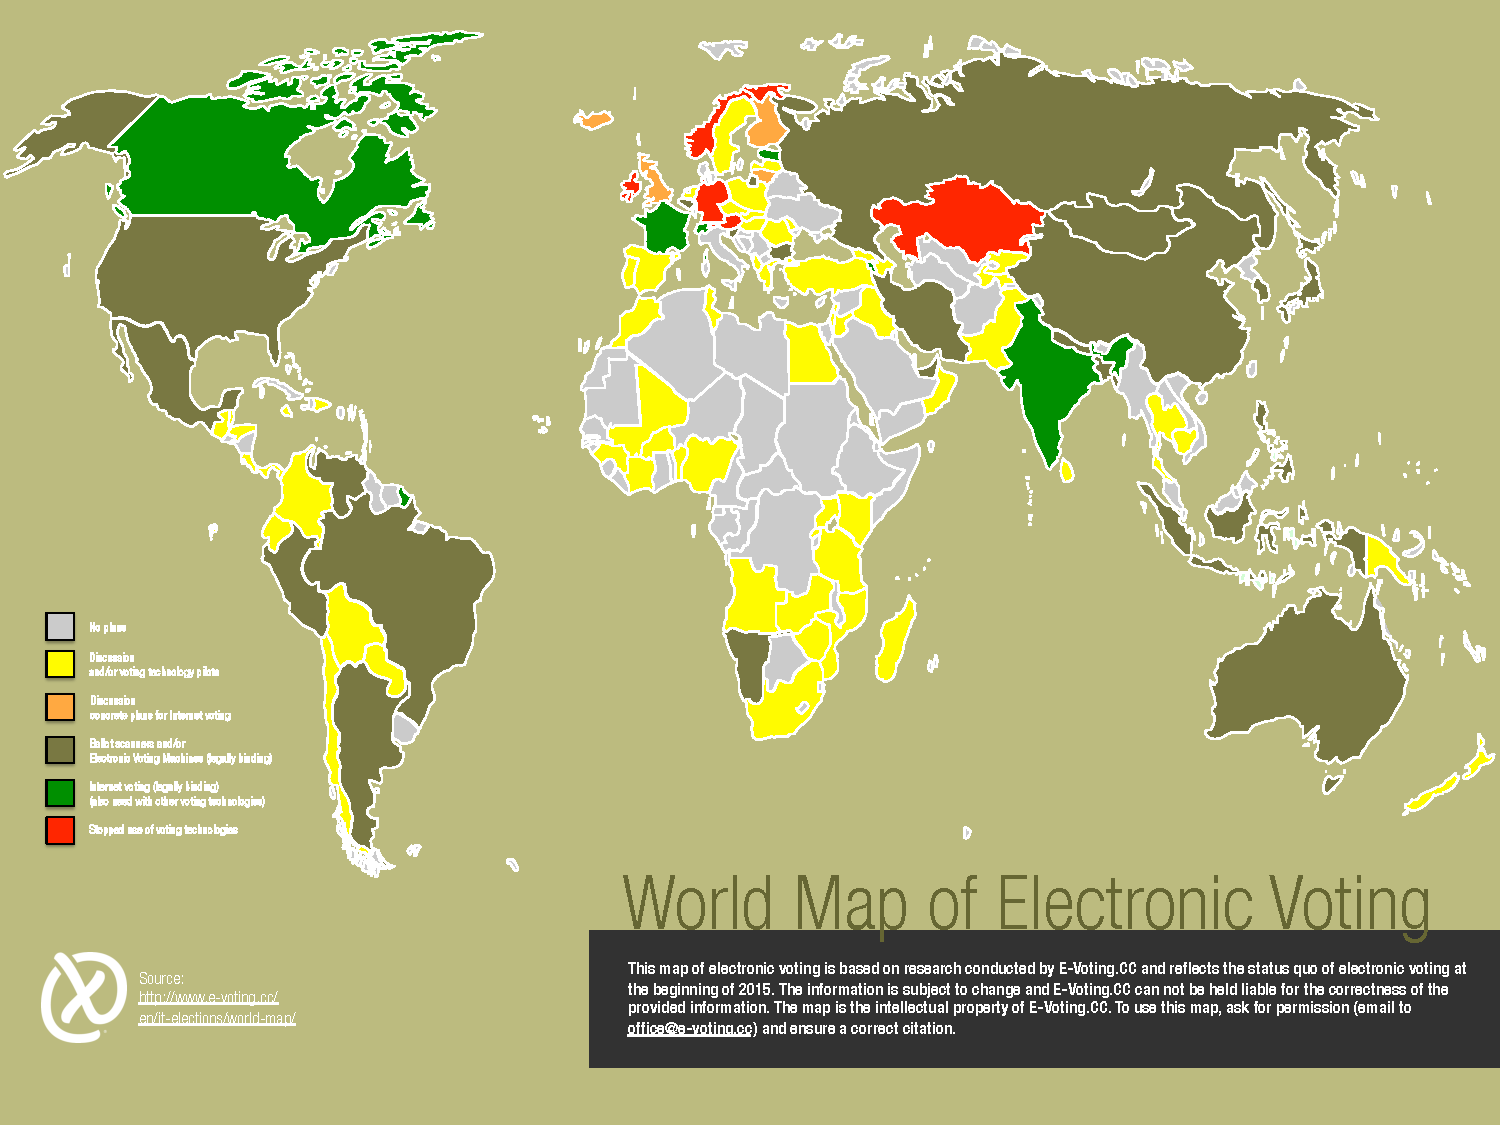
\includegraphics[scale=0.5]{e-voting_worldmap_2015.pdf}
	\caption{World map of Electronic Voting}
	\label{fig:world_electronic_voting_map}
	\end{center}
  \end{figure}  
  The world can be divided into five broad categories according to 
  the usage of electronic voting\footnote{https://www.e-voting.cc/en/it-elections/world-map}
  \ref{fig:world_electronic_voting_map}: i) No electronic voting (Grey Area), ii)
  Discussion and/or voting technology pilots (Yellow Area), 
  iii) Discussion and concrete plans for Internet voting (Orange Area),
  iv) Ballot scanners, Electronic Voting Machines, and Internet Voting (Green and Dark Green),
  v) Withdrawn voting technology because of public concern (Red Area) 
%  \begin{enumerate}
%  \item No electronic voting (Grey Area)
%  \item Discussion and/or voting technology pilots (Yellow Area)
%  \item Discussion and concrete plans for Internet voting (Orange Area)
%  \item Ballot scanners, Electronic Voting Machines, and Internet Voting
%        (Green and Dark Green)
%  \item Withdrawn voting technology because of public concern (Red Area) 
%  \end{enumerate}    
%  
 
\textbf{Chapter Outline:}
  Write here a chapter outline
   
%  The input method, form of ballot, used the countries participating 
%  in electronic voting can be broadly divided into three group 
\section{Electronic Voting}
  Electronic voting is already happening, and the
  arguments in favour of electronic voting 
  include increased voter turnout, faster result and lower cost. The Senate 
  election conducted in Western Australia in September 2013 was 
  declared void by the high court because of the loss of 1370 votes. It was 
  re-conducted in April 2014 with the cost of 20 Million 
  AUD with additional  delay in results\footnote{https://www.theguardian.com/world/2014/feb/28/western-australia-senate-election-re-run-to-be-held-on-5-april}. Sometimes, 
  not only cost, but time as well is a major concern.
  \fix{Give a example of seat which took considerable amount 
  of time in declaring result. I can't find it :(}. 
  The advantages of electronic voting 
  look so promising, so why have some countries (Red Area) retracted 
  from electronic voting? Electronic voting makes 
  the process faster, but it has its own layer of added complexities 
  which creates trust issues amongst voters. 
  
  \textbf{Germany:} In the 2005 German election, two voters filed a case in the German 
  Constitutional Court (Bundesverfassungsgericht) because their 
  appeal to scrutinize the election 
  was not heeded by the Committee. They argued that using electronic 
  voting machines to conduct the election was unconstitutional, and 
  these machines could be hacked, hence results of the 2005 election 
  could not be trusted. The case was argued on the grounds 
  of "all essential steps in the elections are subject to 
  public examinability" according to German Constitution 
  (Basic Law for the Federal Republic of Germany). 
  The Court noted that, under the constitution, elections are 
  required to be public in nature:
  
  \textit{"The principle of the public nature of elections requires that all 
  essential steps in the elections are subject to public examinability
  unless other constitutional interests justify an exception. 
  Particular significance attaches here to the monitoring of the 
  election act and to the ascertainment of the election result."}
  \footnote{https://www.bundesverfassungsgericht.de/
  SharedDocs/Entscheidungen/EN/2009/03/cs20090303\_2bvc000307en.html}
 
  \noindent	
  The court did not rule out or prevent the usage of electronic 
  voting machines,  but suggested to make the process more 
  transparent and trustworthy.  
  
  \textit{"The legislature is not prevented from using electronic voting machines 
  in the elections if the constitutionally required possibility of a 
  reliable correctness check is ensured. In particular, voting machines 
  are conceivable in which the votes are recorded elsewhere in addition
   to electronic storage. This is for instance possible with electronic
   voting machines which print out a visible paper report of the vote 
   cast for the respective voter, in addition to electronic recording 
   of the vote, which can be checked prior to the final ballot and is
    then collected to facilitate subsequent checking. Monitoring that is
     independent of the electronic vote record also remains possible when
     systems are deployed in which the voter marks a voting slip and the 
     election decision is recorded simultaneously, 
     or subsequently by electronic means in 
     order to evaluate these by electronic means at the end of the 
     election day."}
  
  \textbf{The Netherlands:}
  The Netherlands were among a few countries who adopted electronic voting 
  in the early nineties (1990), but it did not go very well in the long 
  run and was abolished in 2008 \citep{Jacobs2009}. 
  The reason for abolishing the electronic voting was that   
  the voting machines used in elections were susceptible to many attacks,
  and the results of elections conducted using these machines 
  were not publicly verifiable.  The security flaw was demonstrated by 
  Dutch public foundation, Wij vertrouwen stemcomputers niet
  \footnote{English Translation "We do not trust voting computers"}. 
  They showed that e-voting machines used in election leaks enough
  information to guess the option or choice of a voter, 
  and they can be easily intercepted from 20 to 30 meters
  \footnote{https://www.youtube.com/watch?v=B05wPomCjEY}. 
  
  
  Germany and The Netherlands are some of the rare cases where 
  electronic voting was withdrawn because it was not able to 
  replicate the same trust environment as created by paper 
  ballot systems whereas Australia, and India continued 
  with electronic voting despite having the concerns expressed 
  by researchers about the security of system. 
  
  \textbf{India:}
  India, one of the largest democracies in world, 
  uses electronic voting machines (also known as EVMs) for national 
  and state level  elections despite the fact that many political parties have raised security 
  concern against it. It was already shown in 2010 in the paper 
  Security Analysis of India's Electronic Voting Machines by 
  \cite{Wolchok:2010:SAI:1866307.1866309}  that it 
  is possible to manipulate the election results by replacing the 
  parts of machine with malicious look alike components along with sending 
  them instructions over wireless
  \footnote{https://www.youtube.com/watch?v=ZlCOj1dElDY} 
  \footnote{https://indiaevm.org/}. 
  
%  
%  In recent elections of 2019, the Election Commission of India 
%  announced, to ensure the transparency and 
%  increase the trust of public, that it would use 
%  voter-verified paper audit trail (VVPAT) 
%  one per assembly; however, the Supreme Court of India ordered Election 
%  Commission of India to increase it to five
%  \footnote{https://www.news18.com/news/india/sc-directs-ec-to-increase-vvpat-verification-from-one-evm-to-five-evms-per-constituency-2093363.html}.
%  The Commission  would count VVPAT slips 
%  in randomly selected one polling booth per assembly 
%  constituency in state election and 
%  in one polling booth in each assembly segment for national election, but 
%  now following the Supreme Court decision it has to do the same for 
%  5 randomly selected assembly constituencies/segments. 
%  \fix{Find out if there is a document at Election Commission of 
%  India website and how the process works}. The design of these 
%  machines are closely guard secret,  but it not impossible to gain 
%  access as shown by  Scott Wolchok et. al. It would be more 
%  interesting and beneficial for Indian democracy if Election 
%  Commission of India
%  releases the design to public scrutiny (very much like cryptographic
%  implementation review process). Sometimes these concerns are very 

 \textbf{Australia}
  In March, 2015 state election 
  of New South Wales, Australia, a Internet voting system, iVote,    
  was used and 280,000 votes were cast through it. NSW Election 
  commissioner claimed that it was 
 \textit{
 "It's fully encrypted and safeguarded, it can't be tampered with, 
 and for the first time people can actually after they've voted 
 go into the system and check to see how they voted just to make 
 sure everything was as they intended." }
 \footnote{https://www.abc.net.au/news/2015-02-04/computer-voting-may-feature-in-march-nsw-election/6068290} 

  \noindent
  The voting on iVote 
  opened on Monday March 16 and continued until March 28. On 22 March,
  two security researchers, Vanessa Teague and J. Alex Halderman, 
  announced that iVote has critical security bug, and they demonstrated 
  that it was good enough to steal any ballot. From their paper
  \citep{10.1007/978-3-319-22270-7_3}
  
  \textit{ 
  "While the election was going on, we performed an independent,
   uninvited security analysis of public portions of the iVote 
   system. We discovered critical security flaws that would allow
   a network-based attacker to perform downgrade-to-export 
   attacks, defeat TLS, and inject malicious code 
   into browsers during voting. We showed that an attacker could
   exploit these flaws to violate ballot privacy and steal votes. 
   We also identified several methods by which an attacker could
   defeat the verification mechanisms built into the iVote design." }
  
  \noindent
  Basically New South Wales ran a online election for 6 days on 
  buggy software which was susceptible to many attacks with a possible 
  outcome of tampered ballot without anyone noticing it. 
%  After the 
%  report was published on \textbf{Freedom To Tinker}
%  \footnote{https://freedom-to-tinker.com/2015/03/22/ivote-vulnerability/}, 
%  it caught the attention of media and NSW Election Commissioner 
%  Ian Brightwell on ABC
%	\footnote{https://www.abc.net.au/news/2015-03-23/ivote-security-hack-allowed-change-of-vote-security-expert-says/6340168}  
%   acknowledged the problem with further adding 
%  that it is fixed and now safe to use.
%  
%  "We are confident however that the system is yielding the outcome that
%   we actually initially set out to yield, and that is that the
%   verification process is not telling us any faults are in the system." 
%   
%   I admire the confidence of NSW Election Commissioner, but, I believe, 
%   he had no idea about the gravity of situation. It is not uncommon 
%   on dark web \footnote{http://mvfjfugdwgc5uwho.onion} to sell zero 
%   day vulnerabilities for couple of thousand of dollars.  
%   Put this story in footnote. FBI paid 
%   some undisclosed amount of money to professional hacker to buy zero 
%   day vulnerability which allowed them to 
%   unlock the iPhone of San Bernardino  shooter without triggering 
%   the security measure of iPhone which would wipe all the data. 
   
   There are various factors for these debacles, but one of the most 
   common denominator among all these debacles
   which contributed significantly  is the software used in the election process. 
   These software are developed via a process called software engineering process 
   or software development process, and it varies from company to company, 
   but  roughly, it translates to  requirement 
   gathering, software design, implementation, testing, and maintenance. 
   During this whole process of transforming a vague idea into 
   concrete software, testing the is the only phase which deals 
   with software bugs. However, testing is not adequate measure
   for instilling the confidence in software that it is bug free 
   as stated by Edsger W. Dijkstra:
   \textit{ "Program testing can be used to show the presence of bugs, 
    but never to show their absence!"}. Besides, these software 
    are closely guarded secrets and their source 
   code in not open for general public because of commercial 
   interests of companies 
   \footnote{https://www.aec.gov.au/information-access/foi/2014/files/ls4912-1.pdf}.
   
%   In general, the software development process follows  
%   
%   
%  The reason for  this problem can be attributed to software development practises 
%   followed by the companies who develop these software. These practices 
%   vary from company to company, but roughly they are requirement 
%   gathering, software design, implementation, testing, and maintenance. 
%   During this whole process of transforming a vague idea into 
%   concrete software, testing the is the only phase which deals 
%   with software bugs. However, testing is not adequate measure
%   for instilling the confidence in software that it is bug free 
%   as stated by 
%    Edsger W. Dijkstra 
%    "Program testing can be used to show the presence of bugs, 
%    but never to show their absence!". Besides, these software 
%    are closely guarded secrets and their source 
%   code in not open for general public because of commercial 
%   interests of companies.
%   
%   \subsection{Problem Statement}
%   [Find some reference]
%   One of the common denominator among all these state of art 
%   electronic voting or, rather I say debacles, is 
%   the software used in voting process were buggy. These bugs 
%   could lead to a possible compromise system; hence, we can not 
%   trust these software for their result. In worst case, 
%   there would be no guarantee for privacy 
%   and verifiability of election. 
%   
%   In this thesis, we address the problem of software bugs, 
%   
%   
%   
%  
%   
   In the next section, I will discuss that software testing 
   in not adequate for electronic voting software, and we should 
   prove the  correctness of software
   by using formal verification techniques \cite{BECKERT2014115}.
   I will argue that  having a rigorous software development methodology would alleviate 
	the bug problem with few case studies as a supporting evidence. The success of these 
	case studies should be a good motivation for us to 
	adopt formal method for electronic voting software development. 
   
   
   \subsection{Software Bugs : A Formal Method Approach}

%	\fix {Write here the software bug story and how they could have 
%	been avoided by formal verification. Pave the path to 
%	next part of Estonia}     
%	
%	
%	One of the biggest reason for having a little or no trust at all 
%	in electronic voting is a mere possibility of bugs in 
%	the deployed software could lead to incorrect result.  
%	In this section, I will argue that 
%	having a rigorous software development methodology would alleviate 
%	the bug problem with few case studies. The success of these 
%	case studies would be good enough motivation, I hope, for us to 
%	adopt their approach for electronic voting software development. 
%    [Add a emphasis here that there is no silver bullet, but 
%     innovations attacking essential complexity could lead to
%     significant improvements. Fred Brooks 
%     There  is  no magic bullet technique that solves all the 
%     problems, but a coordinated  application  of  a  
%     range  of  techniques  does work.] 	

  
	
%	\subsubsection{Common Criteria Software Certification}    	
%	[software certification]
%	EAL 1 : Functionally Tested 
%	EAL 7 : Formally Verified Design and Tested
%	but it leaves the gap between Design and implementation.
%	Write something good about it, but this is not rigorous because 
%	it leaves the gap between design and implementation ? 
%	https://ts.data61.csiro.au/projects/TS/l4.verified/numbers.pml	
%	MicroSoft NT kernel was EAL4 certified, but it was full of bugs, 
%	so it's certainly not the approach we should take for electronic 
%	voting.		    
		    
%	\subsubsection{Formally Verified Software}
	Formal verification has been successfully applied in many areas ranging 
	from verified C compilers CompCert[reference], verified ML compiler
	CakeML, Vellvm: Verifying the LLVM, verified cryptography 
	Fiat-crypto, verified 
	operating system CertiKOS and SeL4, verified theorem prover Milwa, 
	verified crash resistant file system FSCQ, verified distributed system 
	Verdi, mechanisation of Four Color Theorem, Fundamental Theorem of 
	Algebra, and Kepler Conjecture. One thing I would like to emphasize 
	is that none of these are toy project, and it takes years 
	to develop and verify them e.g. SeL4 took 5 years [find the time and 
	cost of these projects]. Also, some of these products 
	are used in commercially e.g CompCert is used by AIRBUS, and MTU
	\footnote{https://www.absint.com/compcert/} and Fiat-crypto is used 
	in Google's BoringSSL library for elliptic-curve arithmetic 
	\footnote{https://deepspec.org/entry/Project/Cryptography}. 
	The very basic question to ponder about using formal method to develop 
	software:  i) Does it achieve the goal given the cost and effort ? ii) Are these 
	software bug free ?
%	The most basic question to ponder  
%	is that is it worth of efforts and does it achieve its 
%	 goals [may be more elegant sentence] ? Are 
%	these software developed formally bug free ? 
   
	One of the most basic way to 
	break the software is generating random tests and throwing it to 
	the software under consideration \cite{Miller:1990:ESR:96267.96279}.
	\cite{Yang:2011:FUB:1993316.1993532} developed random 
	C program generator and used these programs to test various 
	compilers. In three years of its usage, they have found 325 unknown
	bugs in various compiler including GCC
	\footnote{https://embed.cs.utah.edu/csmith/gcc-bugs.html} and LLVM
	\footnote{https://embed.cs.utah.edu/csmith/llvm-bugs.html}; however, 
	they could not find any bug in verified component of CompCert. 
	In their own words \cite{Yang:2011:FUB:1993316.1993532},
	
	\textit{"The striking thing about our CompCert results is that the middle-end 
	bugs we found in all other compilers are absent. As of early 2011,
	the under-development version of CompCert is the only compiler we
	have tested for which Csmith cannot find wrong-code errors. This is
	not for lack of trying: we have devoted about six CPU-years to the
	task. The apparent unbreakability of CompCert supports a strong
	argument that developing compiler optimizations within a proof
	framework, where safety checks are explicit and machine-checked,
	has tangible benefits for compiler users."}
	
	Formal verification is not only helpful in proving the correctness, 
	but sometimes, it helps in uncovering the bugs in design of
	software. ACL2, a Lisp based theorem prover, helped 
	AMD to uncover a floating point bug in Athelon processor which 
	has survived 80 million floating point test cases! 
	In the paper, Milestones from the Pure Lisp theorem proverto ACL2
	\cite{Moore2019}, Moore, one of the developer of ACL2, writes:
	
	\textit{"When AMD developed their translator 
	from their register-transfer language (in which designs
	are expressed) to ACL2 functions they ran 80 million 
	floating point test cases through the ACL2 model of 
	Athlon’s FMUL and their own RTL simulator. However, the 
	subsequent proof attempt exposed bugs not covered by the
	test suite. These bugs were fixed before the Athlon was 
	fabricated."}
	
	There are numerous instances where formal verification 
	was very handy, and it caught the lurking bugs in design in early 
	stage which could never have been found by testing. For 
	electronic voting software used in democratic election, where we 
	can't afford to lose a single ballot or miscalculation 
	or any undefined behaviour, should be developed 
	rigorously using formal method techniques.  
	
	
% \subsection{Electronic Voting Properties}
%   	\subsubsection{Privacy}
%         Give some overview to Encryption, Decryption and 
%         Zero knowledge proof
%       
%   	\subsubsection{Verifiability}
%       Verifiability in electronic voting context is that outcome 
%       any one verify the outcome of election based on produced data. 
%       
		
 \subsection{Verification and Verifiability}
%   \fix{How to make electronic voting more successful ?}   
   Formal verification is useful in producing the 
   bug free code, but it does not answer the question that 
   why should a voter trust the formally verified system. We solely can not 
   establish the trust in the system based on argument of 
   formal verification.  I would call formal verification a necessary, but not the sufficient condition. 
   Combing both \emph{verification} of the
	computer software that counts votes, and
	\emph{verifiability} of individual counts are critical for
	building trust in an election process.  Given the mission-critical importance of
	 correctness of vote-counting,
	both for the legal integrity of the process and for
	building public trust,  it is imperative to replace the
	currently used black-box software for vote-counting with a
	counterpart that is both verified and produces 
	evidence, we call it certificate or scrutiny sheet, which can later be used to certify
	the outcome of election.
	
In order to ascertain that the results of a verified program are
indeed correct, one therefore needs to
\begin{enumerate}
\item read, understand and validate the formal specification: is it
error free, and does it indeed reflect the intended functionality?
\item scrutinize the formal correctness proof: has the verification
been carried out with due diligence, is the proof complete or does
it rely on other assumptions?
\item ensure that the computing equipment on which the (verified)
program is executed has not been tampered with or is otherwise
compromised, and finally
\item ascertain that it was indeed the verified program that was
executed in order to obtain the claimed results.
\end{enumerate}

\noindent
The trust in correctness of any result rests on all items above.
The second two items are
more problematic as they require trust in the integrity of
equipment, and individuals, both of which can be hard to ascertain
once the computation has completed. The
first two trust requirements can be met by publishing both the
specification and the correctness proof so that the specification
can be analysed, and the proof can be replayed. Both need a
considerable amount of expertise but can be carried out by (ideally
more than one group of) domain experts. Trust in the correctness of the
result can still be achieved if a large enough number of domain
experts manage to replicate the computation, using equipment they
know is not compromised, and running the program they know has been
verified. As such, trust in \emph{verified} computation mainly rests
on a relatively small number of domain experts.
   
   
\subsection{Legal Aspects of Verification and Verifiability}
Any system for counting votes in democratic elections needs to
satisfy at least three conditions: (1) each person's vote must be
counted accurately, according to a mandated procedure, (2) the
system and process should be subjectively trusted by the electorate,
(3) there should be an objective basis for such trust, or in other
words the system must be trustworthy. While subjective trust cannot
be guaranteed through greater transparency \cite{ONeill:2002:QT}, transparency about
both the voting system and the actual counting of the vote in a
particular election are important in reducing errors and ensuring an
accurate count, promoting public trust and providing the evidential
basis for demonstrated trustworthiness. In particular, it is a lack
of transparency that has been the primary source of criticism of
existing systems, both in the literature
\cite{Carrier:2012:VCT,Conway:2017:ANS} and among civil
society organisations \cite{Vogl:2012:WWC} (for example,
\texttt{blackboxvoting.org} and
\texttt{trustvote.org}). International commitment to transparency is also
demonstrated through initiatives such as the Open Government
Partnership. Another important concept referred to both in the
literature and by civil society organisations is public
accountability, which requires both giving an “account” or
explanation to the public and when called on (for example, in court)
as well as being held publicly responsible for failures.
Transparency is thus a crucial component of accountability, although
the latter will involve other features (such as enforcement
mechanisms) that are beyond the scope of this paper. 

There are two contexts in which transparency is important in the
running of elections. First, there should be transparency in Hood's
sense \cite{Hood:2001:T} as to the process used in elections generally. This is
generally done through legislation with detailed provisions
specifying such matters as the voting method to be used 
%(as noted above, the Schulz method is not generally used in public office
%elections)
 as well as the requirements for a vote to count as valid.
In a semi-automated process, this requires a combination of
legislation (instructions to humans) and computer code (instructions
to machines). The second kind of transparency, corresponding to
Meijer’s use of the term \cite{Meijer:2014:T}, is required in relation to the
performance of these procedures in a specific election. In a manual
process, procedural transparency is generally only to
intermediaries, the scrutineers, who are able to observe the
handling and tallying of ballot papers in order to monitor officials
in the performance of their tasks. While the use of a limited number
of intermediaries is not ideal, measures such as allowing
scrutineers to be selected by candidates (eg Commonwealth Electoral
Act 1918 (Australia) s 264) promote public confidence that the
procedure as a whole is unbiased. However imperfect, procedural
transparency reduces the risk of error and fraud in execution of the
mandated procedure and enhances trust. 

Electronic vote counting ought to achieve at least a similar level
of transparency along both dimensions as manual systems in order to
promote equivalent levels of trust. Ideally, it would go further
given physical limitations (such as the number of scrutineers
able to fit in a room) apply to a smaller part of the process. The
use of a verified, and fully verifiable system is transparent in both senses, with members of
the public able to monitor both the rules that are followed
and the workings and performance of the system in a particular
instance. 

First, the vote counting procedure needs to be transparent. For
electronic vote counting, the procedure is specified in both
legislation (which authorises the electronic vote counting
procedure) and in the software employed. The use of open source code
ensures that the public has the same level of access to instructions
given to the computer as it has to legislative commands given to
election officials. The use of open source code is crucial as is
demonstrated through a comparison of different jurisdictions of
Australia. In Australia, for example, the Federal Senate and NSW
state election vote counting are based on proprietary black box
systems while the Australian Capital Territory uses open source
eVACS software
\cite{AEC:2013:LMM,Conway:2017:ANS,EA:2016:EVC}. This has
significant impact on the ability of researchers to detect errors
both in advance of elections and in time to correct results
\cite{Conway:2017:ANS}.
Private verification systems have been less successful, in both
Australia and the US, in providing equivalent protection against
error to open source software
\cite{Carrier:2012:VCT,Conway:2017:ANS}. Further, private
verification provides a lower level of public transparency than the
use of manual systems which rely on public legislation (instructions
to humans) as the primary source of vote counting procedures
\cite{Carrier:2012:VCT}. It
should also be noted that there are few public advantages in secrecy
since security is usually enhanced by adopting an open approach
(unless high quality open source vote counting software were
unavailable), and private profit advantages are outweighed by the
importance of trust in democratic elections. 

Second, verifiability provides a method of ascertaining the
correctness of
results of a specific election. External parties are able to check a
certificate to confirm that the counting process has operated
according to the rules of the voting procedure.
% (here, the Schultz method). 
Under a manual process, tallying and counting can only be confirmed by a small number of scrutineers directly observing human
officials. The certification process allows greater transparency not
limited to the number of people able to fit within a physical space,
although we recognise that physical scrutiny is still required for
earlier elements of the voting and vote counting process (up to
verification of optical scanning of ballots). Certification reduces
the risk of error and fraud that would compromise accuracy and
provides an evidence-base for trustworthiness. It is also likely to
increase subjective public trust, although this will require
engagement with the public as to the nature of verification
involved. While it is likely that in practice checking will be
limited to a small group with the technical expertise,
infrastructure and political interest to pursue it, knowledge as to
the openness of the model is likely to increase public trust.
Currently in Australia, neither open source nor proprietary vote
counting systems provide an equivalent level of procedural
transparency for monitoring the count in a particular election (for
example, compare Commonwealth Electoral Act 1918 (Australia) s
273A). 

Ultimately, legislation, computer code (where relevant) and
electoral procedures need to combine to safeguard an accurate count
in which the public has justified confidence. The verification and
verifiability measures suggested here go further to ensure this than
current methods used in Australia and, as far as we are aware,
public office elections around the world.


   		
		
   
%   \subsection{Estonia : Success Story}
%   \fix{Write the details which made Estonia a success story}
%	Estonia Internet voting is far from being perfect, but so far 
%	it has sustained all the attempts to hack it. So what made 
%	Estonian system successful despite the obvious problems. 
%	They always keep their software updated [Read more on it and
%	write a nice narrative]
	

  
    
%    Write here about Trust is highly dependent on Culture. How
%    corruption affects it and how do we perceive trust.    
%   
%   	
%    
%    In Germany and The Netherlands, paper ballot is trusted more, 
%    while Nigeria trusts more in electronic voting. 
%    
%	In paper ballot election, voters assumes that once he cast his
%	ballot and put it in to ballot box and once it reached to counting 
%	booth then his ballot will be included in count. 
%	Every party appoints his own team of scrutineers to observe 
%	the counting, so trust here is not assumed, but enforced. 
%		
%	  
%      What is the meaning of trust in electronic voting. 
%       It should allow voters and election observers to verify, 
%       independently of the hardware and software running the 
%       election, that votes have been recorded, tallied and 
%       declared correctly.
%       
%       Write here about why do we need Privacy and Verifiability.
%       How do we achieve them.
       
%       
%     
%   \subsection{Legislation and Accountability}
%    Write here about what legislation states and how accountability 
%    is enforced. 
%   	 
  
	       
    
   \subsection{Scrutiny Sheet}
   Scrutiny sheet is the tabulation of relevant data to ascertain the result of election. 
   The idea of requiring that computations provide not only results, but also a witness attesting
    to the correctness of the computation is not new,
	and has been put forward in \citep{89397},  
	Certifying-algorithms\footnote{https://people.mpi-inf.mpg.de/~mehlhorn/ftp/CertifyingAlgorithms.pdf},
	\cite{Arkoudas:2005:DRC}, and in \cite{Schurmann:2009:EET} in the context
	of electronic voting.   In general, the idea of computation is that a computable function \textit{f}, it takes 
	a input \textit{x} and produces output \textit{y}; however, in case of certified computation, 
	the computable function \textit{f} on the given input \textit{x}, not only produces the output \textit{y},
	but it also produces a witness \textit{w} for the fact that $ f (x) = y$.
	
	
\begin{tikzpicture}
\draw (0,0) rectangle (10,10) node[pos=0.5] {program for f};
\end{tikzpicture}


  \noindent
   Below is simple piece of Haskell code, but the choice of language does not matter as long as it 
   produces a certificate, which computes the greatest common divisor 
   of two numbers with a certificate.  The first component of computation is the result and second one 
   the certificate. 
   \begin{verbatim}
   gcdWithCertificate :: Integer -> Integer -> (Integer, String)
   gcdWithCertificate a b
    | b == 0 = (a, "gcd " ++ show a ++ " 0 = " ++ show a)
    | otherwise = 
      let (rgcd, rcertificate) = gcdWithCertificate b (mod a b) in
      (rgcd, "gcd " ++ show a ++ " " ++ show b ++ "\n" ++ rcertificate)
   \end{verbatim}
  
   \noindent 
   After running the program on the concrete input 144 and 89, it produces the result and certificate (below).
   \begin{verbatim}
     gcd 144 89
     -------------
     gcd 89 55
     -------------
          .
          .
          .
     -------------
     gcd 2 1
     -------------
     gcd 1 0 
     -------------
        1
   \end{verbatim}
   
   
   In order to verify the correctness of computation of greatest common divisor ($\gcd$), all we need to do is 
   check  that one of the rule, give below, is applicable at every stage of computation:
   \begin{enumerate}
   \item  $\forall$ x, $\gcd$ x 0 = x
   \item $\forall$ x y, $\gcd$ x y = $\gcd$ y (mod x y)
   \end{enumerate}
   
   \noindent 
  It is very crucial to know that the primary purpose of checkers are to verify the 
  correctness of computation, hence, it is important that they 
  should be: i) correct, and ii) simple.  We will discuss more about certificate checking 
  in chapter Software Independence,  and we will argue that why formal verifying the checkers is 
  a good idea to achieve the correctness.  We will also present a case study of 
  formally verified checker for \textit{IACR 2018} election.
  
  
    
   
\section{Summary}
We reiterate that to maximise trust, reliability and auditability of electronic vote counting, we
need both approaches, verification and verifiability, to be combined. To ensure
(universal) verifiability, we advocate that vote-counting programs
do not only compute a final result, but additionally produce an
independently verifiable certificate that attests to the correctness
of the computation, together with a formal verification that
valid certificates indeed imply the correct determination of
winners. Given a certificate-producing vote-counting program, external
parties or stakeholders can then satisfy themselves to the
correctness of the count by checking the certificate.    

In the next chapter, I will  briefly discussion about Coq theorem, and why did we choose it 
to formalize the Schulze method.

\fix{Can I introduce Write Hilbert's idea of mathematical formalism/Frege}

A proof assistant is a computer program which assists users in development of mathematical proofs. The idea of 
developing mathematical proofs using computer goes back to Automath (automating mathematics)
[cite Automath] and LCF [cite Logic for computation] project. The 
Automath project (1967 until the early 80's)  was initiative of De Bruijn, and the aim of the project was to develop
a language for expressing mathematical theories which can be verified by aid of computer.  Automath was first 
practical project to exploit the Curry-Howard isomorphism (proofs-as-programs and formulas-as-types)
 [reference here]. DeBruijn  was likely unaware of this correspondence, and he almost re-invented it 
 ([Wiki entry on Curry-Howard]). Many researchers refers Curry-Howard isomorphism as 
 Curry-Howard-DeBruijn isomorphism. Automath project can be seen as the precursor of
 proof assistants NuPrl [cite here] and Coq [cite coq].   Some other notable  proof assistants are 
 LCF (Logic for Computable Functions)  [cite Milner?], Mizar [cite], Nqthm/ACl2 [cite], PVS [cite], 
 HOL (a family of tools derived from LCF theorem prover), Agda [cite], and Lean [cite].


In this chapter, I will give a overview of theoretical foundation of 
Coq thorem prover i.e. Calculus of Construction and  
Calculus of Inductive Construction, followed by Dependent type 
and how it leads to 
correct by construction (paradigm?) with a example of dependent 
typed lambda calculus. I will also discuss distinction between Type and Prop 
and how it affects the code extraction, a feature for extracting 
certified functional programs from specification proofs, and the 
specification language Gallina. Finally, I would 
argue that why should we trust the Coq proofs even though it does not 
match or look like a mathematical proof.




\section{Coq: Interactive Theorem prover}
\label{sec:problemstatement}
\fix{explain here a about Coq. What is Coq ?}
The Coq proof assistant  is an interactive theorem prover based on
underlying theory of Calculus of 
Inductive Construction [Cite Pualine Mohring]  which itself is an 
augmentation of Calculus of Construction 
[cite Huet and Coquand] with inductive data-type.  
 

\subsection{Calculus of Construction}
\subsection{Calculus of Inductive Construction}
\fix{Flesh out the details of 
 Calculus of construction and Inductive construction}
 \fix{Write here about syntax and semantics of CIC}
 
 

 
\subsection{Dependent Types}
    Type system is a wide spectrum ranging from Scheme where 
    type is runtime concept to Haskell to Coq 
    
    \subsubsection{Example : Dependent Type Lambda Calculus}
     Lambda Calculus encoded in Coq using Inductive data type. 
     
 \subsubsection{Correct by Construction}
 \fix{Combing program with proofs leads to one stop solution, mainly 
     correct by construction}
  Well typed program can't go wrong. 
  Give a example of dependent type lambda calculus(Dirk's white board)
  Hello World is dependent type Vector 
 \subsubsection{Type vs. Prop : Code Extraction}
 \fix{explain here the difference between Prop and Types. How it affects 
  the code extraction }
  It's good starting point to tell the reader that we have two definitions, 
  one in type and other in prop. Why ? Because Type computes, but it's
  not very intuitive for human inspection while Prop does not compute, 
  but it's very intuitive for human inspection. We have connected that 
  the definition expressed in Type is equivalent to Prop definition. 
 
 \subsubsection{Gallina : The Specification Language}
  The example, dependent type lambda calculus, I gave in previous 
  section was encoded in Coq's specification language Gallina. 
  Gallina is a highly expressive specification 
  language for development of mathematical theories and proving the    
  theorems about these  theories; however, writing proofs in Gallina
  is very tedious and cumbersome. It's not suitable for large proof 
  development, and to ease the proof development Coq also provides 
  tactics.  The user interacting with Coq theorem prover applies these 
  tactics to build the  Gallina term  which otherwise would  
  be very laborious.
  
  \fix{Can I give a simple example to demonstrate the difference 
     between proof build directly in Gallina and proof build using 
     tactics}
  
 
  

 
 \subsection{Trusting Coq proofs}
  The fundamental question for trusting the Coq proofs is two fold: 
  i) is the logic (CIC) sound ?, ii) is the implementation correct ?. 
  The logic has already been reviewed by many peers and proved correct 
  using some meta-logic. The 
  Coq implementation itself can be partitioned into two parts: 
  i) Validity Checker (Small kernel), 
  ii) Tactic language to build the proofs.
  We lay our trust in validity checker, because it's small kernel. If there
  is bug in tactic language which often is the case then build proof would 
  not pass the validity checker.  
  
  Try to write here how Fuzzer failed to find bugs in Compcert. 
  
\section{Summary} 
  Paves the path to Cryptography. 
    
\section{Cryptography}
    Write some basic crypto stuff
    
    \subsection{Homomorphic Encryption}
     Add the details of 
     homomorphic encryption 
     \subsubsection{El-Gamal Encryption Scheme}
        Give both additive and multiplicative
     \subsubsection{Pallier Encryption Scheme}
        Write some description
     \subsection{Commitment Schemes}   
        \subsubsection{Hash Based Commitment Scheme}
        \subsubsection{Discrete Logarithm Based Commitment Scheme}
         Pedersen's Commitment Scheme
     \subsection{Zero Knowledge Proof}
  		Details from 
  	 \subsection{Sigma Protocol : Efficient Zero Knowledge Proof}
  



\section{Summary}










%
%%\label{sec:problemstatement}
%Now I give a small example which defines natural number, addition of two natural numbers, and 
%proof that addition over natural number is commutative.   We can define 
%natural number in Coq using inductive data type (listing 1.1), addition of the natural numbers 
%(listing 1.2), and proof that addition of natural numbers is commutative written in Gallina (listing 1.3).
%
%\begin{lstlisting}[language=haskell, numbers=none, basicstyle=\ttfamily, 
%caption=Inductive Data Type for Natural Numbers,  captionpos=b, xleftmargin=.1\textwidth]
%
%Inductive Natural : Type :=
% | O : Natural
% | Succ : Natural -> Natural
%
%\end{lstlisting}
%
%More precisely, the interpretation is that Natural is a inductive type with two constructors: i) O representing zero,
%and ii) Succ representing successor which takes a Natural number and gives next Natural number.
%
%\fix{Change the Addition into infix symbol + and use + in proofs. It will convey the idea more clearly}
%\begin{lstlisting}[language=haskell, numbers=none, basicstyle=\ttfamily,  caption=Addition function for Natural Numbers,  captionpos=b, xleftmargin=.1\textwidth]
%
% 
%Fixpoint Addition (n m : Natural) : Natural :=
%  match n with
%  | O => m
%  | Succ n' => Succ (Addition n' m)
%  end.
%
%(* Notation for Addition. Now we can use + instead of 
%   writing Addition *)
%Notation "x + y" := (Addition x y)
%            (at level 50, left associativity).
%\end{lstlisting}
%
%We define the addition by pattern matching on first argument \textbf{n}. When \textbf{n} is 
%O (zero), then we sum is \textbf{m}, and if \textbf{n} is \textbf{Succ n'}, then sum is successor of 
%\textbf{n' +  m}.
%
%\begin{lstlisting}[language=haskell, numbers=none, basicstyle=\ttfamily,  caption=Addition function for Natural Numbers,  captionpos=b, xleftmargin=.1\textwidth]
%
%Theorem Addition_by_zero : forall (n : Natural), n + O = n.
%  refine (fix IHa (n : Natural) : n + O = n :=
%            match n as nz return (nz + O = nz) with
%            | O => eq_refl
%            | Succ n' =>
%              let IHn' := IHa n' in
%              eq_ind_r (fun m => Succ m = Succ n') eq_refl IHn'
%            end).
%Qed.
%
%  
%Lemma Successor_addition : forall (n m : Natural),
%    Succ (n + m) = n + (Succ m).
%  refine
%    (fix IHn (n : Natural) : forall m : Natural,
%        Succ (n + m) = n + (Succ m) :=
%       match n as nz return (forall m : Natural,
%                                Succ (nz + m) =
%                                nz + (Succ m)) with
%       | O => fun m : Natural => eq_refl
%       | Succ n' =>
%         fun m : Natural =>
%           eq_ind (Succ (n' + m))
%                  (fun t => Succ (Succ (n' + m)) = Succ t)
%                  eq_refl (n' + (Succ m)) (IHn n' m)
%       end).
%Qed.
%     
%
%    
%Theorem Addition_is_commutative :
%  forall (n m : Natural), n +  m = m + n.
%  refine
%    (fix IHn (n : Natural) : forall m : Natural,
%        n + m = m + n :=
%       match n as nz return (forall m : Natural,
%                                nz + m =
%                                m + nz) with
%       | O => fun m : Natural => eq_ind_r (fun t => m = t)
%                                      eq_refl
%                                      (Addition_by_zero m)
%       | Succ n' =>
%         fun m  =>
%           eq_ind (Succ (m + n'))
%                  (fun t => Succ (n' + m) = t)
%                  (eq_ind_r (fun t => Succ t = Succ (m + n'))
%                            eq_refl (IHn n' m))
%                  (m + (Succ n'))
%                  (Successor_addition m n')
%       end).
%Qed.
%
%
%\end{lstlisting}
%
%
%We need two additional Lemma:
% i) $Addition\_by\_zero$, a proof of n + 0 = 0,
% and ii) $Successor\_addition$, a proof of Succ (n + m) = n + (Succ m) 
% to prove that addition on Natural is commutative ($Addition\_is\_commutative$), 
% 
% One thing that can't escape from the reader's eyes is that the proofs written in Gallina is verbose, and they don't 
% appear anywhere compared to a proof that would have been written by a mathematician. Well, we can lift the burden 
% of verbosity by using tactics provided by Coq; however, there is no universally accepted solution in Coq community 
% for second problem. There has been some research in declarative style proof writing 
% \footnote{www-verimag.imag.fr/~corbinea/ftp/publis/bricks-poster.pdf}, but it is not widely practised in Coq 
% community. The proof of addition on Natural is commutative re-written using tactics (Listing 1.4)
% 
% 
% \begin{lstlisting}[language=haskell, numbers=none, basicstyle=\ttfamily,  caption=Addition function for Natural Numbers,  captionpos=b, xleftmargin=.1\textwidth]
%
%Lemma Addition_by_zero : forall (n : Natural), n + O = n.
%  induction n; cbn; [auto | rewrite IHn; auto].
%Qed.
%
%
%Lemma Successor_addition : forall (n m : Natural),
%    Succ (n + m) = n + (Succ m).
%Proof.
%  induction n; intros m;
%    cbn; [auto | rewrite <- IHn; auto].
%Qed.
%
%
%Theorem Addition_is_commutative :
%  forall (n m : Natural), n +  m = m + n.
%Proof.
%  induction n; intro m;
%    [rewrite Addition_by_zero |
%     rewrite <- Successor_addition;
%     rewrite <- IHn]; auto.
%Qed.
%
%\end{lstlisting}
%
%Section~\ref{sec:motivation} xxxx.\\
%
%
%Section~\ref{sec:relatedwork} yyyy.\\
%
%
%%\section{Motivation}
%%\label{sec:motivation}
%
%
%%\section{Related work}
%%\label{sec:relatedwork}
%%You may reference other papers. For example: 
%%Generational garbage collection~\citep{LH:83,Moon:84,Ungar:84} is perhaps the
%%single most important advance in garbage collection since the first collectors
%%were developed in the early 1960s. (doi: "doi" should just be the doi part, not
%%the full URL, and it will be made to link to dx.doi.org and resolve.
%%shortname: gives an optional short name for a conference like PLDI '08.)
%%
%%
%%
%%
%%
%%\section{Summary}
%%Summary what you discussed in this chapter, and mention the story in next
%%chapter. Readers should roughly understand what your thesis takes about by only reading
%%words at the beginning and the end (Summary) of each chapter.
%
%
%
